%! Author = wolfram_e_laube
%! Date = 06.05.24

\item[(b)]
\section{Task (b): Fourier Transform and Spectrum Visualization}

\subsection{Fourier Transform of $x(t)$}
Given the signal $x(t) = \sin(2\pi 4000 t) + \sin(2\pi 6000 t)$, we calculate the Fourier transform, which reveals delta functions at the frequencies of the sinusoidal components:
$$
X(f) = \frac{1}{2i} \left(\delta(f - 4000) - \delta(f + 4000) + \delta(f - 6000) - \delta(f + 6000)\right)
$$
This expression indicates that the spectrum of $x(t)$ consists of spikes at $\pm 4000$ Hz and $\pm 6000$ Hz.

\subsection{Spectrum Visualization and Sampling Effects}
The spectrum is then visualized, taking into account the sampling frequency $f_s = 10,000$ Hz, which leads to periodic replication of the spectrum. The replication and the combination of these spectra due to sampling are illustrated to show how aliasing could affect the resultant digital signal $x[n]$. The effects are demonstrated using a Python script that plots the original and shifted spectra within the range $-f_s$ to $+f_s$.

\begin{figure}[h]
    \centering
    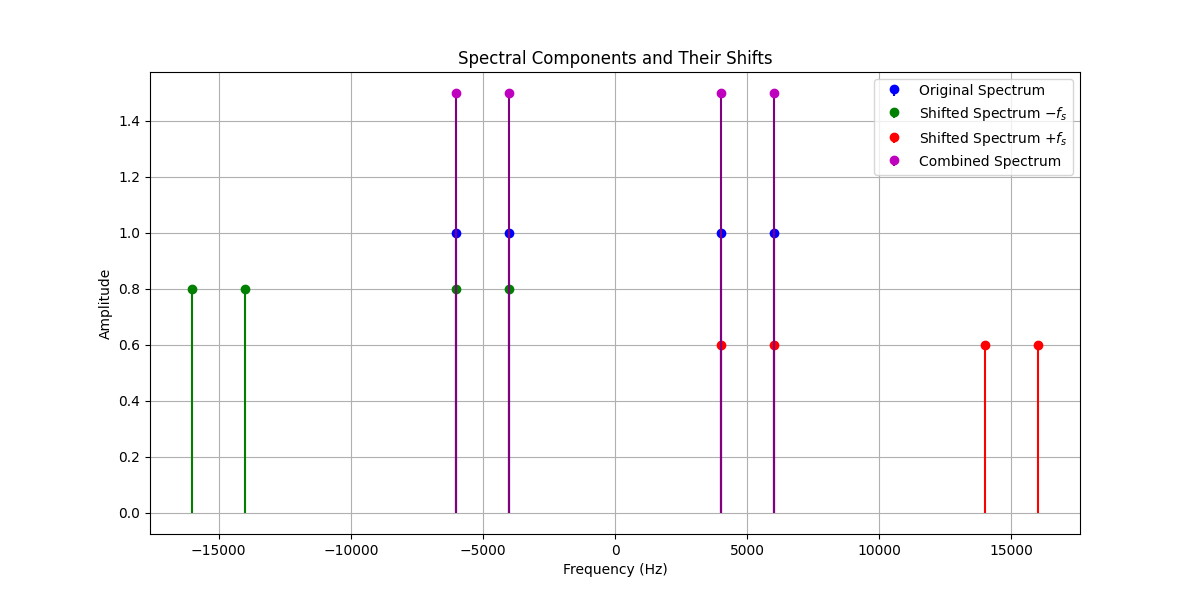
\includegraphics[width=0.49\textwidth]{fig/ex1_b_plot}
    \caption{Spectrum of \(x(t)\)}
    \label{fig:ex1_b_plot}
\end{figure}

The shifted spectrum plot will show the spectral shifts due to the sampling frequency and illustrate the overlapping spectra.